\section{Figures}

\begin{figure}[ht]

\centering \includegraphics[width=1.0\textwidth]{figures/fig1}

\caption{The post-processing pipeline. The T₂-weighted imaging (T₂w) data set
is standardized while the monoexponential and kurtosis models are applied to
diffusion weighted imaging (DWI) data set. The T₂ relaxation values are obtained
using a two parameter monoexponential function. Subsequently, the features are
calculated using T₂w and parametric maps. The feature selection is performed
by choosing 1\% of the features with highest AUC\@. Then with the selected
features a logistic regression model is fitted and used to predict the lesion's
Gleason score group.}\label{fig:pipeline}

\end{figure}


\begin{figure}[ht]

\centering \includegraphics[width=1.0\textwidth]{figures/fig2}

\caption{An example of a whole mount prostate histological section~(A), with
corresponding parametric maps for ADCₘ~(B), ADCₖ~(C), K~(D), T₂w~(E)
and T₂~(F). This is from patient number 43 in Table S1. The two lesions are
outlined; their Gleason scores are 4+3 (lower, in posterolateral region) and 3+4
(upper, in anterior region).}\label{fig:pmap}

\end{figure}


\begin{figure}[ht]

\centering \includegraphics[width=1.0\textwidth]{figures/fig3}

\caption{An example of prostate texture feature maps extracted from DWI
parametric maps (ADCₘ, ADCₖ, K), T₂-weighted imaging (T₂w), and parametric map
of T₂ relaxation values (T₂). Source image type, window size, and texture
descriptor parameters are shown above the images. The two lesions are outlined;
their Gleason scores are 4+3 (lower) and 3+4 (upper).}\label{fig:tmap}

\end{figure}


\begin{figure}[ht]

\centering 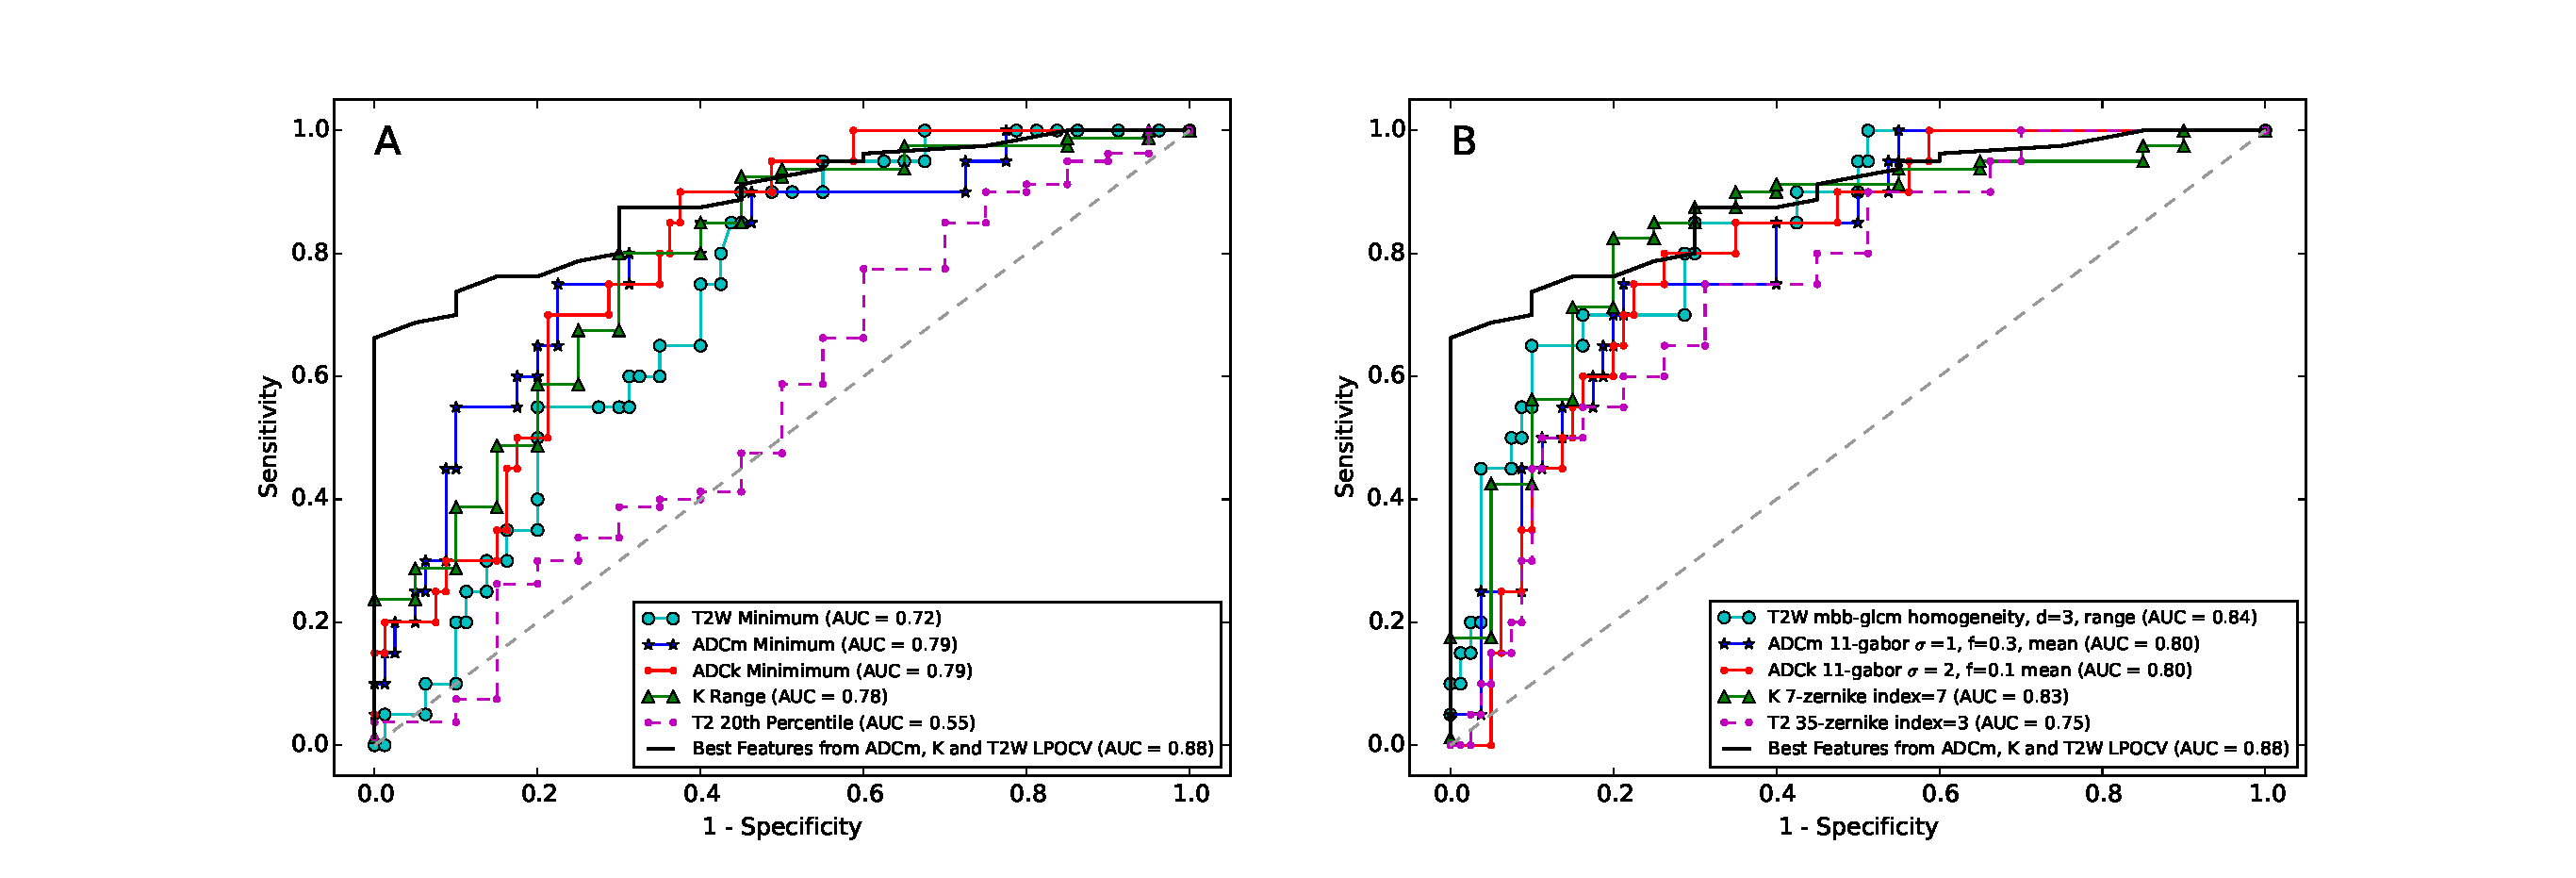
\includegraphics[width=1.0\textwidth]{figures/fig4}

\caption{The ROC curves for the best statistical feature (A) and the best
texture feature (B) within each image type (T₂w, ADCₘ, ADCₖ, K, T₂). The final
model of the best selected features from ADCₘ, K, and T₂w obtained using L1
regularized logistic regression and validated with leave-pair-out
cross-validation (LPOCV) is also included in both A and~B.}\label{fig:roc}

\end{figure}
